\whiteBGstarBegin
\setcounter{section}{0}
\section{Trắc nghiệm}
\begin{enumerate}[label=\bfseries Câu \arabic*:]
	
	
	\item \mkstar{1}
	
	\cauhoi
	{Điện năng được đo bằng
		\begin{mcq}(2)
			\item vôn kế.
			\item công tơ điện.
			\item ampe kế.
			\item tĩnh điện kế.
		\end{mcq}
		
	}
	\loigiai
	{	\textbf{Đáp án: B.}
		
		Điện năng được đo bằng công tơ điện.
	}
	\item \mkstar{1}
	
	\cauhoi
	{Công suất điện được đo bằng đơn vị nào sau đây?
		\begin{mcq}(2)
			\item Niu-tơn (N).
			\item Jun (J).
			\item Oát (W).
			\item Culông (C).
		\end{mcq}
		
	}
	\loigiai
	{	\textbf{Đáp án: C.}
		
		Công suất điện được đo bằng đơn vị Oát (W).
	}
	\item \mkstar{1}
	
	\cauhoi
	{Công suất của nguồn điện được xác định bằng
		\begin{mcq}
			\item lượng điện tích mà nguồn điện sản ra trong 1 giây.
			\item công mà lực lạ thực hiện khi dịch chuyển 1 đơn vị điện tích dương ngược chiều điện trường bên trong nguồn điện.
			\item lượng điện tích chạy qua nguồn điện trong 1 giây.
			\item công của lực điện thực hiện khi dịch chuyển 1 đơn vị điện tích dương chạy trong mạch điện kín trong 1 giây.
		\end{mcq}
		
	}
	\loigiai
	{	\textbf{Đáp án: D.}
		
		Công suất của nguồn điện được xác định bằng công của lực điện thực hiện khi dịch chuyển 1 đơn vị điện tích dương chạy trong mạch điện kín trong 1 giây.
	}
	\item \mkstar{1}
	
	\cauhoi
	{Khi một động cơ điện đang hoạt động thì điện năng được biến đổi thành
		\begin{mcq}
			\item năng lượng cơ học.
			\item năng lượng cơ học và năng lượng nhiệt.
			\item năng lượng cơ học, năng lượng nhiệt và năng lượng điện trường.
			\item năng lượng cơ học, năng lượng nhiệt và năng lượng ánh sáng.
		\end{mcq}
		
	}
	\loigiai
	{	\textbf{Đáp án: B.}
		
		Khi một động cơ điện đang hoạt động thì điện năng được biến đổi thành năng lượng cơ học và năng lượng nhiệt.
	}
	\item \mkstar{2}
	
	\cauhoi
	{Cho mạch điện gồm một pin $\SI{1.5}{V}$ có điện trở trong $\SI{0.5}{\Omega}$ nối với mạch ngoài là một điện trở $\SI{2.5}{\Omega}$. Cường độ dòng điện trong toàn mạch là
		\begin{mcq}(4)
			\item $\SI{3}{A}$.
			\item $\SI{0.6}{A}$.
			\item $\SI{0.5}{A}$.
			\item $\SI{2}{A}$.
		\end{mcq}
		
	}
	\loigiai
	{	\textbf{Đáp án: C.}
		
		Áp dụng định luật Ôm toàn mạch:
		$$I=\dfrac{\calE}{R + r} = \SI{0.5}{A}.$$
	}
	\item \mkstar{2}
	
	\cauhoi
	{Một mạch điện gồm có nguồn là một pin $\SI{9}{V}$, điện trở mạch ngoài $\SI{4}{\Omega}$, cường độ dòng điện trên toàn mạch là $\SI{2}{A}$. Điện trở trong của nguồn là
		\begin{mcq}(4)
			\item $\SI{0.5}{\Omega}$.
			\item $\SI{4.5}{\Omega}$.
			\item $\SI{1}{\Omega}$.
			\item $\SI{2}{\Omega}$.
		\end{mcq}
		
	}
	\loigiai
	{	\textbf{Đáp án: A.}
		
		Áp dụng định luật Ôm toàn mạch:
		$$I=\dfrac{\calE}{R + r} \Rightarrow r = \SI{0.5}{\Omega}.$$
	}
	\item \mkstar{2}
	
	\cauhoi
	{Cho mạch điện gồm hai pin có suất điện động và điện trở trong của mỗi pin là $\SI{1.5}{V} - \SI{0.5}{\Omega}$ mắc nối tiếp rồi nối với mạch ngoài là một điện trở $\SI{2}{\Omega}$. Cường độ dòng điện toàn mạch là
		\begin{mcq}(4)
			\item $\SI{3}{A}$.
			\item $\SI{0.6}{A}$.
			\item $\SI{1}{A}$.
			\item $\SI{2}{A}$.
		\end{mcq}
		
	}
	\loigiai
	{	\textbf{Đáp án: C.}
		
		Suất điện động của bộ nguồn:
		$$\calE_\text b = 2\calE = \SI{3}{V}.$$
		
		Điện trở trong của bộ nguồn:
		$$r_\text b = 2 r = \SI{1}{\Omega}.$$
		
		Cường độ dòng điện toàn mạch:
		$$I=\dfrac{\calE_\text b}{R + r_\text b} = \SI{1}{A}.$$
	}
	\item \mkstar{2}
	
	\cauhoi
	{Một mạch điện gồm có nguồn là một pin $\SI{9}{V}$, điện trở trong $\SI{0.5}{\Omega}$ và mạch ngoài gồm hai điện trở $\SI{8}{\Omega}$ mắc song song. Cường độ dòng điện trên toàn mạch là
		\begin{mcq}(4)
			\item $\SI{2}{A}$.
			\item $\SI{4.5}{A}$.
			\item $\SI{1}{A}$.
			\item $\xsi{\dfrac{18}{33}}{A}$.
		\end{mcq}
		
	}
	\loigiai
	{	\textbf{Đáp án: A.}
		
		Điện trở tương đương mạch ngoài:
		$$R = \dfrac{\SI{8}{\Omega}}{2} = \SI{4}{\Omega}.$$
		
		Cường độ dòng điện toàn mạch:
		$$I=\dfrac{\calE}{R + r} = \SI{2}{A}.$$
	}
	\item \mkstar{2}
	
	\cauhoi
	{Hai bóng đèn sợi đốt cùng công suất định mức, có các hiệu điện thế định mức lần lượt là $U_1$ và $U_2$. Xác định tỉ số điện trở $\dfrac{R_1}{R_2}$ của hai bóng đèn theo $U_1$ và $U_2$.
		\begin{mcq}(4)
			\item $\dfrac{R_1}{R_2} = \left(\dfrac{U_1}{U_2}\right)^2$.
			\item $\dfrac{R_1}{R_2} = \dfrac{U_2}{U_1}$.
			\item $\dfrac{R_1}{R_2} = \dfrac{U_1}{U_2}$.
			\item $\dfrac{R_1}{R_2} = \left(\dfrac{U_2}{U_1}\right)^2$.
		\end{mcq}
		
	}
	\loigiai
	{	\textbf{Đáp án: A.}
		
		Từ biểu thức tính điện trở theo công suất định mức: $R=\dfrac{U_\text{đm}^2}{\calP}$, suy ra:
		$$\dfrac{R_1}{R_2} = \left(\dfrac{U_1}{U_2}\right)^2.$$
	}
	\item \mkstar{2}
	
	\cauhoi
	{Tính hiệu suất của một bếp điện nếu sau $t=20$ phút nó đun sôi được $\SI{2}{l}$ nước từ nhiệt độ ban đầu $\SI{20}{\celsius}$. Biết rằng cường độ dòng điện chạy qua bếp là $I=\SI{3}{A}$, hiệu điện thế đặt vào là $U=\SI{220}{V}$.
		\begin{mcq}(4)
			\item $H=\SI{75}{\percent}$.
			\item $H=\SI{85}{\percent}$.
			\item $H=\SI{95}{\percent}$.
			\item $H=\SI{65}{\percent}$.
		\end{mcq}
		
	}
	\loigiai
	{	\textbf{Đáp án: B.}
		
		Nhiệt lượng (công có ích):
		$$Q=mc \Delta t = \SI{672000}{J}.$$
		
		Điện năng tiêu thụ (công toàn phần):
		$$A=UI t = \SI{792000}{J}.$$
		
		Hiệu suất của bếp điện:
		$$H=\dfrac{Q}{A} = \SI{85}{\percent}.$$
	}
	\item \mkstar{2}
	
	\cauhoi
	{Cho mạch điện như hình vẽ.
		\begin{center}
			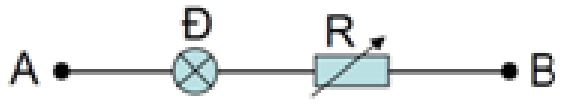
\includegraphics[scale=0.6]{../figs/VN11-2021-PH-TP017-1}
		\end{center}
	
	Hiệu điện thế giữa hai đầu đoạn mạch là $\SI{15}{V}$, trên đèn có ghi $\SI{12}{V} - \SI{6}{W}$, điện trở dây nối không đáng kể. Hãy xác định giá trị của biến trở để đèn sáng bình thường.
		\begin{mcq}(4)
			\item $R=\SI{1}{\Omega}$.
			\item $R=\SI{3}{\Omega}$.
			\item $R=\SI{6}{\Omega}$.
			\item $R=\SI{9}{\Omega}$.
		\end{mcq}
		
	}
	\loigiai
	{	\textbf{Đáp án: C.}
		
		Điện trở của đèn:
		$$R_\text{đ} = \dfrac{U_\text{đm}^2}{\calP} = \SI{24}{\Omega}.$$
		
		Để đèn sáng bình thường thì cường độ dòng điện qua mạch là
		$$I=\dfrac{\calP_\text{đm}}{U_\text{đm}} = \SI{0.5}{A}.$$
		
		Vậy giá trị biến trở cần tìm là
		$$I=\dfrac{U}{R + R_\text{đ}} \Rightarrow R = \SI{6}{\Omega}.$$
	}
	\item \mkstar{3}
	
	\cauhoi
	{Một bóng đèn $\SI{100}{V} - \SI{50}{W}$ được mắc vào mạng điện $\SI{240}{V}$. Để đèn sáng bình thường thì cần phải mắc nối tiếp với điện trở $R$ có giá trị
		\begin{mcq}(4)
			\item $R=\SI{280}{\Omega}$.
			\item $R=\SI{880}{\Omega}$.
			\item $R=\SI{200}{\Omega}$.
			\item $R=\SI{120}{\Omega}$.
		\end{mcq}
		
	}
	\loigiai
	{	\textbf{Đáp án: A.}
		
		Điện trở của đèn:
		$$R_\text{đ} = \dfrac{U_\text{đm}^2}{\calP} = \SI{200}{\Omega}.$$
		
		Để đèn sáng bình thường thì cường độ dòng điện qua mạch là
		$$I=\dfrac{\calP_\text{đm}}{U_\text{đm}} = \SI{0.5}{A}.$$
		
		Vậy giá trị điện trở cần tìm là
		$$I=\dfrac{U}{R + R_\text{đ}} \Rightarrow R = \SI{280}{\Omega}.$$
	}
	\item \mkstar{3}
	
	\cauhoi
	{Một nguồn điện có suất điện động $\calE$, điện trở trong $r$ mắc với mạch ngoài là điện trở $R$. Hiệu suất của nguồn điện là $H=\SI{80}{\percent}$. Tỉ số giữa điện trở trong của nguồn ($r$) và điện trở mạch ngoài ($R$) là
		\begin{mcq}(4)
			\item $\SI{0.80}{}$.
			\item $\SI{0.20}{}$.
			\item $\SI{0.40}{}$.
			\item $\SI{0.25}{}$.
		\end{mcq}
		
	}
	\loigiai
	{	\textbf{Đáp án: D.}
		
		Áp dụng công thức tính hiệu suất của nguồn:
		$$H=\dfrac{U}{\calE} = \dfrac{IR}{I(R+r)} = \dfrac{R}{R + r} = \SI{80}{\percent} \Rightarrow \dfrac{r}{R} = \dfrac{1}{4} = \SI{0.25}{}.$$
	}
	\item \mkstar{3}
	
	\cauhoi
	{Một động cơ điện một chiều có điện trở thuần của các cuộn dây là $r=\SI{4}{\Omega}$, mắc nối tiếp với một điện trở $R=\SI{8}{\Omega}$. Tất cả được mắc vào nguồn điện có hiệu điện thế không đổi và bằng $\SI{24}{V}$. Động cơ khi đó hoạt động bình thường và cường độ dòng điện qua động cơ là $\SI{0.5}{A}$. Công suất điện năng chuyển hóa thành cơ năng ở động cơ là
		\begin{mcq}(4)
			\item $\SI{3}{W}$.
			\item $\SI{12}{W}$.
			\item $\SI{10}{W}$.
			\item $\SI{9}{W}$.
		\end{mcq}
		
	}
	\loigiai
	{	\textbf{Đáp án: D.}
		
		Gọi $\calP_\text{đc}$ là công suất điện năng chuyển hóa thành cơ năng của động cơ.
		
		Áp dụng định luật Ôm:
		$$I=\dfrac{U}{R_\text{đc} + R + r} = \SI{0.5}{A} \Rightarrow R_\text{đc} = \SI{36}{\Omega}.$$
		
		Vậy công suất điện năng chuyển hóa thành cơ năng của động cơ là
		$$\calP_\text{đc} = I^2 R_\text{đc} = \SI{9}{W}.$$
	}
	\item \mkstar{3}
	
	\cauhoi
	{Để nạp điện cho một ắc quy có suất điện động $\calE_2 = \SI{6}{V}$, điện trở trong $r_2 = \SI{0.4}{\Omega}$, người ta dùng nguồn điện một chiều có suất điện động $\calE_1 = \SI{12}{V}$, điện trở trong $r_1=\SI{0.2}{\Omega}$ và một biến trở $R$ mắc nối tiếp với ắc quy. Điều chỉnh biến trở đến giá trị $R=\SI{11.4}{\Omega}$, tính công suất điện tiêu thụ ở ắc quy.
		\begin{mcq}(4)
			\item $\SI{9.9}{W}$.
			\item $\SI{9.0}{W}$.
			\item $\SI{3.0}{W}$.
			\item $\SI{3.1}{W}$.
		\end{mcq}
		
	}
	\loigiai
	{	\textbf{Đáp án: D.}
		
		Áp dụng định luật Ôm (với ắc quy đóng vai trò là máy thu):
		$$I=\dfrac{\calE_1 - \calE_2}{R + r_1 + r_2} = \SI{0.5}{A}.$$
		
		Công suất tiêu thụ ở ắc quy bằng tổng công suất nguồn của ắc quy và công suất tỏa nhiệt trên ắc quy:
		$$\calP_2 = \calE_2 I + I^2 r_2 = \SI{3.1}{W}.$$
	}
	\item \mkstar{3}
	
	\cauhoi
	{Cho mạch điện như hình vẽ.
		\begin{center}
			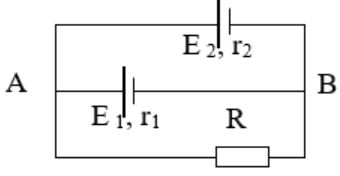
\includegraphics[scale=0.6]{../figs/VN11-2021-PH-TP017-2}
		\end{center}
	
	Trong đó: $\calE_1 = \SI{20}{V}$, $\calE_2 = \SI{32}{V}$, $r_1=\SI{1}{\Omega}$, $r_2=\SI{0.5}{\Omega}$, $R=\SI{2}{\Omega}$. Tìm cường độ dòng điện qua $R$.
		\begin{mcq}(4)
			\item $\SI{4}{A}$.
			\item $\SI{8}{A}$.
			\item $\SI{16}{A}$.
			\item $\SI{12}{A}$.
		\end{mcq}
		
	}
	\loigiai
	{	\textbf{Đáp án: D.}
		
		Hiệu điện thế trên mỗi nhánh:
		$$
		\begin{cases}
			U_\text{AB} = \calE_1 - I_1 r_1 \\
			U_\text{AB} = \calE_2 - I_2 r_2 \\
			U_\text{AB} = IR
		\end{cases}
		$$
		
		Tìm được hệ phương trình:
		$$
		\begin{cases}
			I_1 - \SI{0.5}{} I_2 = \SI{-12}{} \\
			\SI{0.5}{} I_2 + 2I = 32
		\end{cases}
		$$
		
		Mà $I=I_1 +I_2$. Thay vào hệ trên, tìm được $I_1 = \SI{-4}{A}$, $I_2 = \SI{16}{A}$ và $I=\SI{12}{A}$.
	}
	\item \mkstar{3}
	
	\cauhoi
	{Cho mạch điện như hình vẽ.
		\begin{center}
			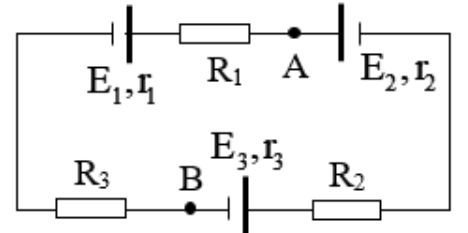
\includegraphics[scale=0.6]{../figs/VN11-2021-PH-TP017-3}
		\end{center}
	
	Cho biết $\calE_1 = \SI{12}{V}$, $r_1=\SI{1}{\Omega}$, $\calE_2 = \SI{6}{V}$, $r_2=\SI{2}{\Omega}$, $\calE_3 = \SI{9}{V}$, $r_3=\SI{3}{\Omega}$, $R_1=\SI{4}{\Omega}$, $R_2=\SI{2}{\Omega}$, $R_3=\SI{3}{\Omega}$. Tính $U_\text{AB}$.
		\begin{mcq}(4)
			\item $U_\text{AB} = \SI{13.6}{V}$.
			\item $U_\text{AB} = \SI{11.6}{V}$.
			\item $U_\text{AB} = \SI{13.2}{V}$.
			\item $U_\text{AB} = \SI{11.2}{V}$.
		\end{mcq}
		
	}
	\loigiai
	{	\textbf{Đáp án: A.}
		
		Áp dụng định luật Ôm cho mạch kín, ta có:
		$$I=\dfrac{\calE_2 + \calE_3 - \calE_1}{R_1 + R_2 + R_3 + r_1 + r_2 + r_3} = \SI{0.2}{A}.$$
		
		Hiệu điện thế $U_\text{AB}$:
		$$U_\text{AB} = \calE_1 + I(R_1 + R_3 + r_1) = \SI{13.6}{V}.$$
	}
	\item \mkstar{3}
	
	\cauhoi
	{Một nguồn điện có suất điện động $\calE = \SI{12}{V}$, điện trở trong $r=\SI{3}{\Omega}$, được mắc với một biến trở $R$ thành mạch kín. Điều chỉnh $R$ để công suất tiêu thụ ở mạch ngoài đạt cực đại. Công suất cực đại đó bằng
		\begin{mcq}(4)
			\item $\SI{144}{W}$.
			\item $\SI{14.4}{W}$.
			\item $\SI{12.0}{W}$.
			\item $\SI{24.0}{W}$.
		\end{mcq}
		
	}
	\loigiai
	{	\textbf{Đáp án: C.}
		
		Áp dụng kết hợp định luật Ôm toàn mạch và biểu thức tính công suất, ta được:
		$$\calP = I^2 R = \dfrac{\calE ^2}{(r+R)^2} R = \dfrac{144 R}{(R+3)^2}.$$
		
		Áp dụng bất đẳng thức Cô-si:
		$$R+3 \geq 2 \sqrt{3 R}.$$
		
		Tính được giá trị cực đại của công suất là
		$$\calP = \dfrac{144 R}{4 \cdot 3R} = \SI{12.0}{W}.$$
	}
	\item \mkstar{3}
	
	\cauhoi
	{Đường đặc trưng Vôn - Ampe của hai vật dẫn có điện trở $R_1$, $R_2$ được cho như hình vẽ.
		\begin{center}
		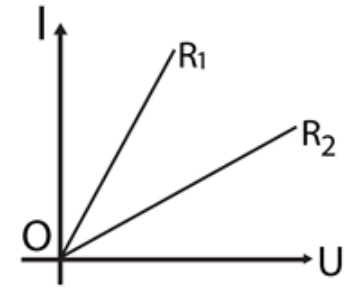
\includegraphics[scale=0.7]{../figs/VN11-2021-PH-TP017-4}
		\end{center}
	
		Chọn kết luận đúng.
		\begin{mcq}(2)
			\item $R_1 < R_2$.
			\item $R_1 > R_2$.
			\item Không thể so sánh $R_1$ với $R_2$.
			\item $R_1=R_2$.
		\end{mcq}
		
	}
	\loigiai
	{	\textbf{Đáp án: A.}
		
		Dựa vào công thức $R=\dfrac{U}{I}$, nhận thấy giá trị này là nghịch đảo của hệ số góc $\tan \alpha$, hay $\dfrac{1}{\tan \alpha} = \dfrac{U}{I}$.
		
		Vậy với $\tan \alpha$ lớn hơn thì $R$ nhỏ hơn. Suy ra $R_1 < R_2$ vì $\tan \alpha_1 > \tan \alpha_2$.
	}
	\item \mkstar{4}
	
	\cauhoi
	{Cho một mạch điện kín gồm nguồn điện có suất điện động $\calE = \SI{12}{V}$, điện trở trong $r=\SI{1.5}{\Omega}$, mạch ngoài gồm điện trở $R_1=\SI{0.5}{\Omega}$ mắc nối tiếp với $R$. Để công suất tiêu thụ trên $R$ đạt cực đại thì giá trị của $R$ là
		\begin{mcq}(4)
			\item $\SI{3}{\Omega}$.
			\item $\SI{2}{\Omega}$.
			\item $\SI{4}{\Omega}$.
			\item $\SI{1}{\Omega}$.
		\end{mcq}
		
	}
	\loigiai
	{	\textbf{Đáp án: B.}
		
		Áp dụng kết hợp định luật Ôm toàn mạch và biểu thức tính công suất, ta được:
		$$\calP = I^2 R = \dfrac{\calE^2}{(r + R_1 + R)^2}R = \dfrac{\calE ^2}{\left(\dfrac{2}{\sqrt{R}} + \sqrt{R}\right)^2}.$$
		
		Áp dụng bất đẳng thức Cô-si:
		$$\dfrac{2}{\sqrt{R}} + \sqrt{R} \geq 2.$$
		
		Vậy giá trị cực đại của công suất đạt được khi $\dfrac{2}{\sqrt{R}} + \sqrt{R} = 2$. Khi đó:
		$$\calP = \dfrac{\calE^2}{2^2} = \SI{36}{W}.$$
		
		Khi đó $R=\SI{2}{\Omega}$.
	}
\end{enumerate}

\whiteBGstarEnd

\loigiai
{
	\begin{center}
		\textbf{BẢNG ĐÁP ÁN}
	\end{center}
	\begin{center}
		\begin{tabular}{|m{2.8em}|m{2.8em}|m{2.8em}|m{2.8em}|m{2.8em}|m{2.8em}|m{2.8em}|m{2.8em}|m{2.8em}|m{2.8em}|}
			\hline
			1.B  & 2.C  & 3.D  & 4.B  & 5.C  & 6.A  & 7.C  & 8.A  & 9.A  & 10.B  \\
			\hline
			11.C  & 12.A  & 13.D  & 14.D  & 15.D  & 16.D  & 17.A  & 18.C  & 19.A  & 20.B  \\
			\hline
		\end{tabular}
	\end{center}
}
\section{Tự luận}
\begin{enumerate}[label=\bfseries Câu \arabic*:]
	\item \mkstar{2}
	
	\cauhoi{
		Một bộ ắc quy có thể cung cấp một dòng điện $\SI{8}{A}$ liên tục trong $\SI{1}{h}$ thì phải nạp lại. Tính suất điện động của ắc quy này nếu trong khoảng thời gian hoạt động trên, nó sản ra một công là $\SI{86.4}{kJ}$.
	}
	
	\loigiai{
		
		Suất điện động của ắc quy này:
		$$\calE = \dfrac{A}{q} = \dfrac{A}{It} = \SI{3}{V}.$$
	}
	
	\item \mkstar{2}
	
	\cauhoi{
		Tính điện năng tiêu thụ và công suất điện khi dòng điện có cường độ $\SI{2}{A}$ chạy qua dây dẫn trong $\SI{1}{h}$. Biết hiệu điện thế giữa hai đầu dây dẫn này là $\SI{6}{V}$.
	}
	
	\loigiai{
		
	Điện năng tiêu thụ:
	$$A= UI t = \SI{43200}{J}.$$
	
	Công suất điện:
	$$\calP = \dfrac{A}{t} = \SI{12}{W}.$$	
	}
	\item \mkstar{2}
	
	\cauhoi{
		Cho ba điện trở giống nhau giá trị $\SI{8}{\Omega}$ gồm hai điện trở mắc song song rồi nối tiếp với điện trở thứ ba. Đoạn mạch này được nối với nguồn điện có điện trở trong $\SI{2}{\Omega}$. Người ta đo được hiệu điện thế giữa hai cực của nguồn là $\SI{12}{V}$. Xác định cường độ dòng điện trong mạch và suất điện động của nguồn điện.
	}
	
	\loigiai{
		
		Điện trở tương đương của mạch ngoài:
		$$R=\dfrac{\SI{8}{\Omega}}{2} + \SI{8}{\Omega} = \SI{12}{\Omega}.$$
		
		Áp dụng công thức xác định hiệu điện thế dựa vào định luật Ôm:
		$$U = \calE - I r \Rightarrow \calE - I r = U \Rightarrow \calE - \dfrac{\calE}{R + r} r = U \Rightarrow \calE= \SI{14}{V}.$$
		
		Cường độ dòng điện trong mạch:
		$$I = \dfrac{\calE}{R + r} = \SI{1}{A}.$$
	}
	\item \mkstar{2}
	
	\cauhoi{
		Một bộ nguồn gồm hai nguồn điện mắc xung đối, nguồn thứ nhất có suất điện động $\calE_1 = \SI{12}{V}$, điện trở trong $r_1=\SI{1}{\Omega}$, nguồn thứ hai có suất điện động $\calE_2 = \SI{4}{V}$, điện trở trong $r_2 = \SI{1}{\Omega}$. Bộ nguồn được mắc với ampe kế có điện trở không đáng kể tạo thành mạch điện kín. Tính hiệu điện thế từ cực dương đến cực âm của nguồn điện $\calE_1$.
	}
	
	\loigiai{
		
		Vì hai nguồn được mắc xung đối nên một trong hai nguồn đóng vai trò là máy thu. Suất điện động của bộ nguồn là
		$$\calE_\text{b} = \SI{12}{V} - \SI{4}{V} = \SI{8}{V}.$$
		
		Điện trở trong của bộ nguồn:
		$$r_\text{b} = r_1 + r_2 = \SI{1}{\Omega} + \SI{1}{\Omega} = \SI{2}{\Omega}.$$
		
		Áp dụng định luật Ôm:
		$$I=\dfrac{\calE_\text b}{R + r_\text b} = \SI{4}{A}.$$
		
		Hiệu điện thế giữa hai cực của $\calE_1$:
		$$U=\calE_1 - I r_1 = \SI{8}{V}.$$
	}
	
\end{enumerate}